%% bare_jrnl.tex
%% V1.4b
%% 2015/08/26
%% by Michael Shell
%% see http://www.michaelshell.org/
%% for current contact information.
%%
%% This is a skeleton file demonstrating the use of IEEEtran.cls
%% (requires IEEEtran.cls version 1.8b or later) with an IEEE
%% journal paper.
%%
%% Support sites:
%% http://www.michaelshell.org/tex/ieeetran/
%% http://www.ctan.org/pkg/ieeetran
%% and
%% http://www.ieee.org/

%%*************************************************************************
%% Legal Notice:
%% This code is offered as-is without any warranty either expressed or
%% implied; without even the implied warranty of MERCHANTABILITY or
%% FITNESS FOR A PARTICULAR PURPOSE! 
%% User assumes all risk.
%% In no event shall the IEEE or any contributor to this code be liable for
%% any damages or losses, including, but not limited to, incidental,
%% consequential, or any other damages, resulting from the use or misuse
%% of any information contained here.
%%
%% All comments are the opinions of their respective authors and are not
%% necessarily endorsed by the IEEE.
%%
%% This work is distributed under the LaTeX Project Public License (LPPL)
%% ( http://www.latex-project.org/ ) version 1.3, and may be freely used,
%% distributed and modified. A copy of the LPPL, version 1.3, is included
%% in the base LaTeX documentation of all distributions of LaTeX released
%% 2003/12/01 or later.
%% Retain all contribution notices and credits.
%% ** Modified files should be clearly indicated as such, including  **
%% ** renaming them and changing author support contact information. **
%%*************************************************************************


% *** Authors should verify (and, if needed, correct) their LaTeX system  ***
% *** with the testflow diagnostic prior to trusting their LaTeX platform ***
% *** with production work. The IEEE's font choices and paper sizes can   ***
% *** trigger bugs that do not appear when using other class files.       ***                          ***
% The testflow support page is at:
% http://www.michaelshell.org/tex/testflow/



\documentclass[journal]{IEEEtran}
%
% If IEEEtran.cls has not been installed into the LaTeX system files,
% manually specify the path to it like:
% \documentclass[journal]{../sty/IEEEtran}

%**** LANGUAGE PACKAGES *****

\usepackage[spanish]{babel}

% Some very useful LaTeX packages include:
% (uncomment the ones you want to load)


% *** MISC UTILITY PACKAGES ***
%
%\usepackage{ifpdf}
% Heiko Oberdiek's ifpdf.sty is very useful if you need conditional
% compilation based on whether the output is pdf or dvi.
% usage:
% \ifpdf
%   % pdf code
% \else
%   % dvi code
% \fi
% The latest version of ifpdf.sty can be obtained from:
% http://www.ctan.org/pkg/ifpdf
% Also, note that IEEEtran.cls V1.7 and later provides a builtin
% \ifCLASSINFOpdf conditional that works the same way.
% When switching from latex to pdflatex and vice-versa, the compiler may
% have to be run twice to clear warning/error messages.



% *** CITATION PACKAGES ***
%
\usepackage{cite}
% cite.sty was written by Donald Arseneau
% V1.6 and later of IEEEtran pre-defines the format of the cite.sty package
% \cite{} output to follow that of the IEEE. Loading the cite package will
% result in citation numbers being automatically sorted and properly
% "compressed/ranged". e.g., [1], [9], [2], [7], [5], [6] without using
% cite.sty will become [1], [2], [5]--[7], [9] using cite.sty. cite.sty's
% \cite will automatically add leading space, if needed. Use cite.sty's
% noadjust option (cite.sty V3.8 and later) if you want to turn this off
% such as if a citation ever needs to be enclosed in parenthesis.
% cite.sty is already installed on most LaTeX systems. Be sure and use
% version 5.0 (2009-03-20) and later if using hyperref.sty.
% The latest version can be obtained at:
% http://www.ctan.org/pkg/cite
% The documentation is contained in the cite.sty file itself.


% *** GRAPHICS RELATED PACKAGES ***
%
\ifCLASSINFOpdf
 \usepackage[pdftex]{graphicx}
 \usepackage{subfigure} % subfiguras
  % declare the path(s) where your graphic files are 
 \graphicspath{ {images/} }
  % and their extensions so you won't have to specify these with
  % every instance of \includegraphics
  \DeclareGraphicsExtensions{.pdf,.jpeg,.png}
\else
  % or other class option (dvipsone, dvipdf, if not using dvips). graphicx
  % will default to the driver specified in the system graphics.cfg if no
  % driver is specified.
  % \usepackage[dvips]{graphicx}
  % declare the path(s) where your graphic files are
  % \graphicspath{{../eps/}}
  % and their extensions so you won't have to specify these with
  % every instance of \includegraphics
  % \DeclareGraphicsExtensions{.eps}
\fi
% graphicx was written by David Carlisle and Sebastian Rahtz. It is
% required if you want graphics, photos, etc. graphicx.sty is already
% installed on most LaTeX systems. The latest version and documentation
% can be obtained at: 
% http://www.ctan.org/pkg/graphicx
% Another good source of documentation is "Using Imported Graphics in
% LaTeX2e" by Keith Reckdahl which can be found at:
% http://www.ctan.org/pkg/epslatex
%
% latex, and pdflatex in dvi mode, support graphics in encapsulated
% postscript (.eps) format. pdflatex in pdf mode supports graphics
% in .pdf, .jpeg, .png and .mps (metapost) formats. Users should ensure
% that all non-photo figures use a vector format (.eps, .pdf, .mps) and
% not a bitmapped formats (.jpeg, .png). The IEEE frowns on bitmapped formats
% which can result in "jaggedy"/blurry rendering of lines and letters as
% well as large increases in file sizes.
%
% You can find documentation about the pdfTeX application at:
% http://www.tug.org/applications/pdftex




% *** MATH PACKAGES ***
%
\usepackage{amsmath}
% A popular package from the American Mathematical Society that provides
% many useful and powerful commands for dealing with mathematics.
%
% Note that the amsmath package sets \interdisplaylinepenalty to 10000
% thus preventing page breaks from occurring within multiline equations. Use:
%\interdisplaylinepenalty=2500
% after loading amsmath to restore such page breaks as IEEEtran.cls normally
% does. amsmath.sty is already installed on most LaTeX systems. The latest
% version and documentation can be obtained at:
% http://www.ctan.org/pkg/amsmath



% *** SPECIALIZED LIST PACKAGES ***
%
\usepackage{algorithmic}
% algorithmic.sty was written by Peter Williams and Rogerio Brito.
% This package provides an algorithmic environment fo describing algorithms.
% You can use the algorithmic environment in-text or within a figure
% environment to provide for a floating algorithm. Do NOT use the algorithm
% floating environment provided by algorithm.sty (by the same authors) or
% algorithm2e.sty (by Christophe Fiorio) as the IEEE does not use dedicated
% algorithm float types and packages that provide these will not provide
% correct IEEE style captions. The latest version and documentation of
% algorithmic.sty can be obtained at:
% http://www.ctan.org/pkg/algorithms
% Also of interest may be the (relatively newer and more customizable)
% algorithmicx.sty package by Szasz Janos:
% http://www.ctan.org/pkg/algorithmicx



\usepackage{xspace} 

% *** ALIGNMENT PACKAGES ***
%
\usepackage{array}
% Frank Mittelbach's and David Carlisle's array.sty patches and improves
% the standard LaTeX2e array and tabular environments to provide better
% appearance and additional user controls. As the default LaTeX2e table
% generation code is lacking to the point of almost being broken with
% respect to the quality of the end results, all users are strongly
% advised to use an enhanced (at the very least that provided by array.sty)
% set of table tools. array.sty is already installed on most systems. The
% latest version and documentation can be obtained at:
% http://www.ctan.org/pkg/array


% IEEEtran contains the IEEEeqnarray family of commands that can be used to
% generate multiline equations as well as matrices, tables, etc., of high
% quality.




% *** SUBFIGURE PACKAGES ***
%\ifCLASSOPTIONcompsoc
%  \usepackage[caption=false,font=normalsize,labelfont=sf,textfont=sf]{subfig}
%\else
%  \usepackage[caption=false,font=footnotesize]{subfig}
%\fi
% subfig.sty, written by Steven Douglas Cochran, is the modern replacement
% for subfigure.sty, the latter of which is no longer maintained and is
% incompatible with some LaTeX packages including fixltx2e. However,
% subfig.sty requires and automatically loads Axel Sommerfeldt's caption.sty
% which will override IEEEtran.cls' handling of captions and this will result
% in non-IEEE style figure/table captions. To prevent this problem, be sure
% and invoke subfig.sty's "caption=false" package option (available since
% subfig.sty version 1.3, 2005/06/28) as this is will preserve IEEEtran.cls
% handling of captions.
% Note that the Computer Society format requires a larger sans serif font
% than the serif footnote size font used in traditional IEEE formatting
% and thus the need to invoke different subfig.sty package options depending
% on whether compsoc mode has been enabled.
%
% The latest version and documentation of subfig.sty can be obtained at:
% http://www.ctan.org/pkg/subfig




% *** FLOAT PACKAGES ***
%
%\usepackage{fixltx2e}
% fixltx2e, the successor to the earlier fix2col.sty, was written by
% Frank Mittelbach and David Carlisle. This package corrects a few problems
% in the LaTeX2e kernel, the most notable of which is that in current
% LaTeX2e releases, the ordering of single and double column floats is not
% guaranteed to be preserved. Thus, an unpatched LaTeX2e can allow a
% single column figure to be placed prior to an earlier double column
% figure.
% Be aware that LaTeX2e kernels dated 2015 and later have fixltx2e.sty's
% corrections already built into the system in which case a warning will
% be issued if an attempt is made to load fixltx2e.sty as it is no longer
% needed.
% The latest version and documentation can be found at:
% http://www.ctan.org/pkg/fixltx2e


%\usepackage{stfloats}
% stfloats.sty was written by Sigitas Tolusis. This package gives LaTeX2e
% the ability to do double column floats at the bottom of the page as well
% as the top. (e.g., "\begin{figure*}[!b]" is not normally possible in
% LaTeX2e). It also provides a command:
%\fnbelowfloat
% to enable the placement of footnotes below bottom floats (the standard
% LaTeX2e kernel puts them above bottom floats). This is an invasive package
% which rewrites many portions of the LaTeX2e float routines. It may not work
% with other packages that modify the LaTeX2e float routines. The latest
% version and documentation can be obtained at:
% http://www.ctan.org/pkg/stfloats
% Do not use the stfloats baselinefloat ability as the IEEE does not allow
% \baselineskip to stretch. Authors submitting work to the IEEE should note
% that the IEEE rarely uses double column equations and that authors should try
% to avoid such use. Do not be tempted to use the cuted.sty or midfloat.sty
% packages (also by Sigitas Tolusis) as the IEEE does not format its papers in
% such ways.
% Do not attempt to use stfloats with fixltx2e as they are incompatible.
% Instead, use Morten Hogholm'a dblfloatfix which combines the features
% of both fixltx2e and stfloats:
%
% \usepackage{dblfloatfix}
% The latest version can be found at:
% http://www.ctan.org/pkg/dblfloatfix




%\ifCLASSOPTIONcaptionsoff
%  \usepackage[nomarkers]{endfloat}
% \let\MYoriglatexcaption\caption
% \renewcommand{\caption}[2][\relax]{\MYoriglatexcaption[#2]{#2}}
%\fi
% endfloat.sty was written by James Darrell McCauley, Jeff Goldberg and 
% Axel Sommerfeldt. This package may be useful when used in conjunction with 
% IEEEtran.cls'  captionsoff option. Some IEEE journals/societies require that
% submissions have lists of figures/tables at the end of the paper and that
% figures/tables without any captions are placed on a page by themselves at
% the end of the document. If needed, the draftcls IEEEtran class option or
% \CLASSINPUTbaselinestretch interface can be used to increase the line
% spacing as well. Be sure and use the nomarkers option of endfloat to
% prevent endfloat from "marking" where the figures would have been placed
% in the text. The two hack lines of code above are a slight modification of
% that suggested by in the endfloat docs (section 8.4.1) to ensure that
% the full captions always appear in the list of figures/tables - even if
% the user used the short optional argument of \caption[]{}.
% IEEE papers do not typically make use of \caption[]'s optional argument,
% so this should not be an issue. A similar trick can be used to disable
% captions of packages such as subfig.sty that lack options to turn off
% the subcaptions:
% For subfig.sty:
% \let\MYorigsubfloat\subfloat
% \renewcommand{\subfloat}[2][\relax]{\MYorigsubfloat[]{#2}}
% However, the above trick will not work if both optional arguments of
% the \subfloat command are used. Furthermore, there needs to be a
% description of each subfigure *somewhere* and endfloat does not add
% subfigure captions to its list of figures. Thus, the best approach is to
% avoid the use of subfigure captions (many IEEE journals avoid them anyway)
% and instead reference/explain all the subfigures within the main caption.
% The latest version of endfloat.sty and its documentation can obtained at:
% http://www.ctan.org/pkg/endfloat
%
% The IEEEtran \ifCLASSOPTIONcaptionsoff conditional can also be used
% later in the document, say, to conditionally put the References on a 
% page by themselves.




% *** PDF, URL AND HYPERLINK PACKAGES ***
%
%\usepackage{url}
% url.sty was written by Donald Arseneau. It provides better support for
% handling and breaking URLs. url.sty is already installed on most LaTeX
% systems. The latest version and documentation can be obtained at:
% http://www.ctan.org/pkg/url
% Basically, \url{my_url_here}.


\usepackage{authblk}

% *** Do not adjust lengths that control margins, column widths, etc. ***
% *** Do not use packages that alter fonts (such as pslatex).         ***
% There should be no need to do such things with IEEEtran.cls V1.6 and later.
% (Unless specifically asked to do so by the journal or conference you plan
% to submit to, of course. )


% correct bad hyphenation here
\hyphenation{op-tical net-works semi-conduc-tor}

% Paquete para saltos del inea
\usepackage[utf8]{inputenc}


% Paquete para utilizar colores
\usepackage{color}

% **** PLOTS PACKAGE ************
\usepackage{pgfplots}
\usepackage{float}
\pgfplotsset{compat=1.16}
\begin{document}
%
% paper title
% Titles are generally capitalized except for words such as a, an, and, %as,
% at, but, by, for, in, nor, of, on, or, the, to and up, which are usually
% not capitalized unless they are the first or last word of the title.
% Linebreaks \\ can be used within to get better formatting as desired.
% Do not put math or special symbols in the title.
\title{ Modelo de lentes interactivos para la visualización y comparación de taxonomías biológicas }
%
%
% author names and IEEE memberships
% note positions of commas and nonbreaking spaces ( ~ ) LaTeX will not break
% a structure at a ~ so this keeps an author's name from being broken across
% two lines.
% use \thanks{} to gain access to the first footnote area
% a separate \thanks must be used for each paragraph as LaTeX2e's \thanks
% was not built to handle multiple paragraphs
%

\author{Manuel Figueroa,\IEEEmembership{ ITCR,}
        Nathalia Gonzalez,\IEEEmembership{ ITCR,}
        Esteban Leandro,\IEEEmembership{ ITCR}}% <-this % stops a space
\affil[]{\textit{MC-7205 Tema Selecto de Investigación}}
\affil[]{\textit{Instituto Tecnológico de Costa Rica}}
\affil[]{\textit{\{mfigueroacr, natgondu, elc790\}@gmail.com}}

% note the % following the last \IEEEmembership and also \thanks - 
% these prevent an unwanted space from occurring between the last author name
% and the end of the author line. i.e., if you had this:
% 
% \author{....lastname \thanks{...} \thanks{...} }
%                     ^------------^------------^----Do not want these spaces!
%
% a space would be appended to the last name and could cause every name on that
% line to be shifted left slightly. This is one of those "LaTeX things". For
% instance, "\textbf{A} \textbf{B}" will typeset as "A B" not "AB". To get
% "AB" then you have to do: "\textbf{A}\textbf{B}"
% \thanks is no different in this regard, so shield the last } of each \thanks
% that ends a line with a % and do not let a space in before the next \thanks.
% Spaces after \IEEEmembership other than the last one are OK (and needed) as
% you are supposed to have spaces between the names. For what it is worth,
% this is a minor point as most people would not even notice if the said evil
% space somehow managed to creep in.



% The paper headers
\markboth{Curso Tema Selecto, ITCR: Maestría en Computación, I Semestre ~2020}%
{Shell \MakeLowercase{\textit{et al.}}: Modelo de lentes interactivos para la visualización y comparación de taxonomías biológicas. }
% The only time the second header will appear is for the odd numbered pages
% after the title page when using the twoside option.
% 
% *** Note that you probably will NOT want to include the author's ***
% *** name in the headers of peer review papers.                   ***
% You can use \ifCLASSOPTIONpeerreview for conditional compilation here if
% you desire.




% If you want to put a publisher's ID mark on the page you can do it like
% this:
%\IEEEpubid{0000--0000/00\$00.00~\copyright~2015 IEEE}
% Remember, if you use this you must call \IEEEpubidadjcol in the second
% column for its text to clear the IEEEpubid mark.



% use for special paper notices
%\IEEEspecialpapernotice{(Invited Paper)}




% make the title area
\maketitle

% As a general rule, do not put math, special symbols or citations
% in the abstract or keywords.
\begin{abstract}
  Se presenta un modelo de visualización alternativo para la comparación de taxonomías biológicas,
  que busca fortalecer el avance logrado en el sistema Diaforá\cite{sancho_diafora}. Permitiendo a los taxónomos
  enfocarse en aspectos importantes de los árboles de clasificación y manteniendo al mismo tiempo un mapa de la totalidad
  de los árboles de taxonomía que están analizando.
  Dicha propuesta pretende ser evaluada por un panel de expertos en taxonomía, para verificar la eficacia de esta extensión al sistema
  Diaforá, de manera similar al análisis presentado en \cite{sancho-study}. 
\end{abstract}

% Note that keywords are not normally used for peerreview papers.
\begin{IEEEkeywords}
\LaTeX\xspace Visualización, Taxonomías biológicas, Diaforá, Enfoque y Contexto.
\end{IEEEkeywords}






% For peer review papers, you can put extra information on the cover
% page as needed:
% \ifCLASSOPTIONpeerreview
% \begin{center} \bfseries EDICS Category: 3-BBND \end{center}
% \fi
%
% For peerreview papers, this IEEEtran command inserts a page break and
% creates the second title. It will be ignored for other modes.
\IEEEpeerreviewmaketitle


\section{Introducción}
% The very first letter is a 2 line initial drop letter followed
% by the rest of the first word in caps.
% 
% form to use if the first word consists of a single letter:
% \IEEEPARstart{A}{demo} file is ....
% 
% form to use if you need the single drop letter followed by
% normal text (unknown if ever used by the IEEE):
% \IEEEPARstart{A}{}demo file is ....
% 
% Some journals put the first two words in caps:
% \IEEEPARstart{T}{his demo} file is ....
% 
% Here we have the typical use of a "T" for an initial drop letter
% and "HIS" in caps to complete the first word.
El problema descrito se deriva de la investigación realizada por los profesores Lilliana 
Sancho Chavarría y Erick Mata Montero del ITCR, como parte  de su  investigación en la comparación
y visualización de taxonomías biológicas \cite{sancho_diafora}.
Las taxonomías biológicas son estructuras donde las especies son clasificadas de
 acuerdo a un sistema jerárquico propuesto por Linnaeus en el siglo 18\cite{linne},
  y que incluye las categorías de dominio, reino, filo o división, clase, orden,
   familia, género y especie.
La información de todos los seres vivientes conocidos se agrupa en
 árboles taxonómicos, que han sido creados y mantenidos por taxónomos a lo largo 
 del mundo durante siglos. La reciente revolución digital ha permitido que gran parte 
 de esa información pueda  ser compartida y revisada por expertos.  
 Debido a la naturaleza dinámica de estos datos es común que los taxónomos se 
 enfrenten a distintas versiones de los datos que pueden ser corregidas y unificadas
  mediante la comparación de árboles taxonómicos. Las herramientas que ayuden a este 
  grupo a analizar e identificar estas diferencias y facilitar el proceso de curación 
  de las taxonomías permitiría un avance significativo en la calidad y fiabilidad de
   las clasificaciones biológicas de los seres vivos.

   %================== TRABAJOS RELACIONADOS

   \section{Trabajos relacionados}
El problema de comparar grandes colecciones de datos es una necesidad común en el campo de la análitica visual \cite{gleicher_2018}, donde se identifica
que a mayor escala se tienen como límite la capacidad cognitiva y perceptiva del usuario.  Para solventar el problema de la escala se sugiere considerar como estrategías para el usuario:
\begin{itemize}
  \item \textbf{Escanear secuencialmente:} el usuario puede examinar los objetos de manera secuencial.
  \item \textbf{Seleccionar un grupo:} el usuario analiza un grupo más pequeño de datos.
  \item  \textbf{Resumir los datos:} presentar al usuario una abstracción que describa los datos.
\end{itemize}
Los trabajos relacionados en comparación de jerarquías de datos biológicos se centran en el estudio de árboles filogenéticos y taxonomías
biológicas.

\section{Análisis del uso de lentes interactivos en taxonomías biológicas}

Uno de los sentidos más importantes de los seres humanos es la visión. 
Ésta es empleada para obtener la información visual del entorno, y en este caso específico la visualización se ha
 convertido en un medio para ayudar a las personas de diversos campos a obtener información relevante sobre los datos. 
 Sin embargo, dado a que el tamaño de los datos aumenta constantemente,
  los enfoques de visualización tienen que resolver el problema de representaciones visuales 
  exponenciales que dificultan la visualización de contenido relevante en una sola imagen de visualización\cite{tominski_gladisch_kister_dachselt_schumann_2016}.
Algunos investigadores como C. Tominski han tratado de abordar el desafío de la visualización con enfoque a través de exploraciones con grandes volúmenes 
de datos. Una de las técnicas para resolver los problemas de visualización son los lentes interactivos,
 una clase de métodos que permiten la exploración de datos con múltiples facetas. 
 Se busca con el uso de lentes interactivos una vista alternativa de los datos presentes en una área 
 específica de la pantalla, con el fin de enfatizar parte de esta información de una manera más clara para los usuarios\cite{tominski_gladisch_kister_dachselt_schumann_2016}.
Los datos estructurados en árboles son comunes en muchas disciplinas; este trabajo se enfocará 
específicamente en las clasificaciones biológicas para la detección de diferencias y detalles relevantes 
en una única pantalla, por ejemplo, los árboles filogenéticos que a diferencia de las categorizaciones 
taxonómicas estudian las relaciones de parentesco entre las especies.
Se han estudiado diferentes técnicas de visualización que permiten enfatizar las similitudes 
y resaltar las diferencias existentes entre los árboles, como árboles de consenso y debido a que estos 
árboles cuentan en promedio con más de 50 nodos es necesario la utilización de estrategias para ordenar 
los árboles de manera automática entre estas se destacan la diferencia mínima de tripletas (MDT), y la
 semejanza máxima de ramas (MBS). Estos algoritmos buscan maximizar el alineamiento de las hojas de los 
 árboles en una comparación cara a cara\cite{inproceedings}.


 \subsection{Lentes Interactivos}

 Según la definición encontrada en \cite{tominski_gladisch_kister_dachselt_schumann_2016}, un lente interactivo es una herramienta ligera, que
 intenta resolver un problema localizado de visualización, alterando temporalmente una parte seleccionada de la representación de los datos.

 También siguiendo el trabajo de Tominski, se definen como propiedades importantes de los lentes interactivos:
 \begin{itemize}
   \item  \emph{Forma:} La forma del lente virtualmente no tiene restricción, sin embargo, es común que muchos sistemas intenten
   emular el modelo de un lente del mundo real, en su mayoría circulares, no obstante esta forma puede adaptarse según la naturaleza de los datos
   que se están explorando. La importancia radica en que el usuario pueda identificar el lente fácilmente y sobre cuales datos quiere que el lente
   realice su función.
   \item \emph{Posición y tamaño:} Se consideran atributos parametrizables, y que el usuario pueda ubicar el lente y ajustar su tamaño sobre
   cualquier parte de los datos en el área de exploración.
   \item \emph{Orientación:} Cuando se emplea el recurso de visualización en tres dimensiones, la orientación toma relevancia en la forma en la que 
   se observan los datos, ya que dependiendo del ángulo de visión del punto de observación el modelo de datos presentado en pantalla puede variar.
 \end{itemize}

 \subsection{Lentes Interactivos para Visualización}
 Las técnicas de lentes son herramientas que nos permiten enfocarnos temporalmente en un punto de interes, un lente es una selección 
 de una visualización base donde se buscan localizar un punto especifico y una vez que se llega al punto de interes
 la visualización vuelve a su estado original. La selección captura lo que debe ser resaltado por un lente. 
 Normalmente el usuario controla la selección a través de movimientos sobre la representación visual de los datos. 
 
 \subsection{Lentes Interactivos para Visualización de Taxonomías}
 La taxonomía tiene su origen en un vocablo griego que significa “ordenación”. Se trata de la ciencia de la clasificación que se aplica en la biología para la ordenación sistemática y jerarquizada de los grupos de animales o plantas.
 Es importante establecer además que la taxonomía está muy en relación con lo que se conoce por el nombre de sistemática. Esta puede definirse como la ciencia que se encarga de llevar a cabo el estudio de las relaciones de parentesco, también llamadas afinidades, 
 que se producen entre las distintas especies.
 En este paper nos enfocaremos en la taxonomía biológica, la cual forma parte de la biología sistemática, dedicada al análisis de las relaciones de parentesco entre los organismos. Una vez que se resuelve el árbol filogenético del organismo en cuestión y se conocen sus ramas evolutivas, 
 la taxonomía se encarga de estudiar las relaciones de parentesco.
 La visión más extendida entiende a los taxones como clados (ramas del árbol filogenético, con especies emparentadas por un antepasado común) que ya fueron asignados a una categoría taxonómica.

El proceso de la taxonomía continúa con la asignación de nombres (de acuerdo a los principios de la nomenclatura), la elaboración de las claves dicotómicas de identificación y la creación de los sistemas de clasificación.

Los taxones permiten clasificar a los seres vivos a partir de una jerarquía de inclusión (cada grupo abarca a otros menores mientras está subordinado a uno mayor). Las categorías fundamentales, desde la más abarcativa hasta la menor, son el 
dominio, el reino, el filo o división, la clase, el orden, la familia, el género y la especie.


\section{Diseño de visualización InterRing para el sistema taxonómico Diáfora}
Las técnicas conocidad como \emph{RSF} o \emph{Radial, space-filling} por sus siglas en inglés,
 tienen ciertas ventajas
para la visualización de jerarquías, utilizan el espacio en pantalla de manera eficiente mientras que proveen una vista intuitiva 
de la estructuras jerárquicas.
\begin{figure}[]
  \centering
  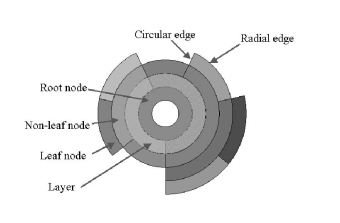
\includegraphics[scale=0.6]{interring}
  \caption{Ejemplo de visualización RSF. Tomado  de \cite{yang_ward_rundensteiner}}
\end{figure}

Haciendo uso de una visualización de tipo \emph{InterRing}\cite{yang_ward_rundensteiner}, que emplea
el concepto de distorción circular extendemos la capacidad actual del sistema \emph{Diaforá} para mantener el contexto
de la estructura jerárquica que esta siendo desplegada en el árbol taxonómico.

\section{Desarrollo del modelo de visualización en el sistema Diaforá}
Según lo investigado en \cite{sancho_diafora}, el método \emph{edge drawing} puede comunicar de manera clara las
diferencias entre dos versiones de una taxonomía. El uso de colores y líneas permite de manera clara detectar los
cambios, además de que la interacción del usuario con la visualización permite enfocarse en aquellos cambios que 
puedan llamar su atención.

La principal desventaja detectada sobre el sistema de visualización \emph{edge drawing} consiste en la pérdida de contexto
de la estructura jerárquica del árbol taxonómico debido a la gran cantidad de nodos presentes una taxonomía.
El propósito de utilizar una visualización \emph{InterRing}\cite{yang_ward_rundensteiner} secundaria pretende apoyar al usuario a conocer
el ámbito local del árbol taxonómico presentando de manera gráfica parte de la jeraquía circundante que puede no ser visible debido a la cantidad de datos
y que para poder visualizarlos requiere que el usuario haga \emph{scroll} sobre la gráfica \emph{edge drawing}.

\begin{figure}[]
  \centering
  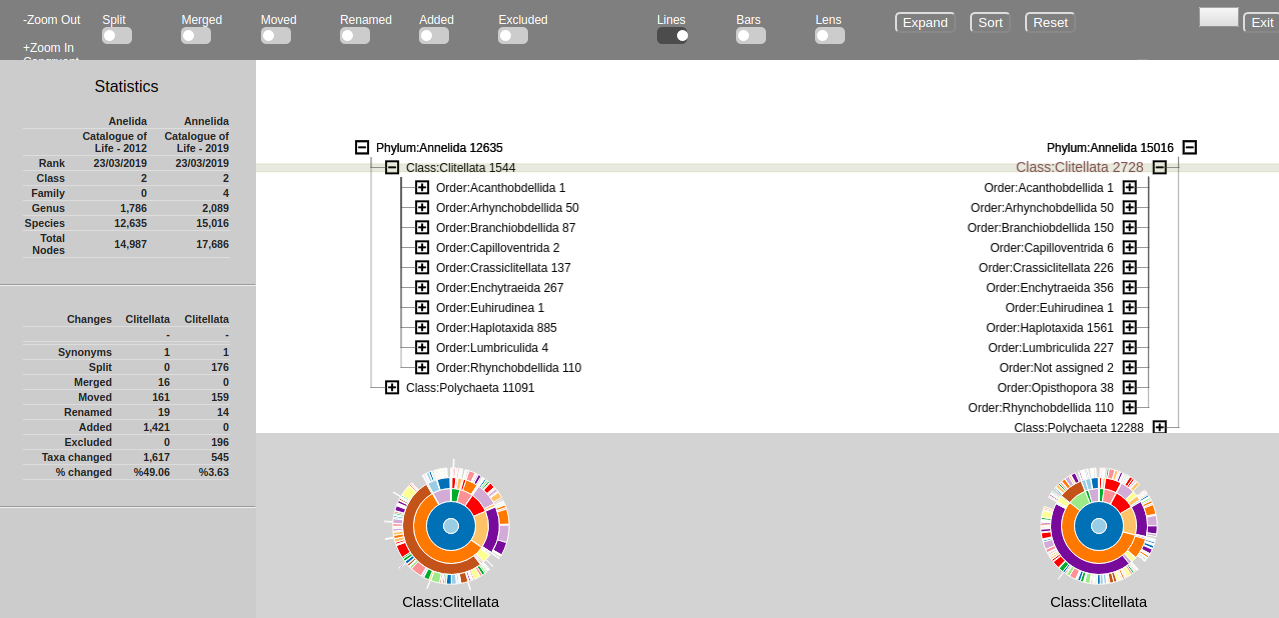
\includegraphics[scale=0.20]{extend_diafora.png}
  \caption{Sistema Diaforá en conjunto con visualización InterRing.}
  \label{}
\end{figure}

El uso del método InterRing permite de manera compacta y simple renderizar una gran cantidad de nodos y permite al usuario navegar sobre las ramas 
del árbol taxonómico y explorar su composición, también al estar sincronizadas ambas gráficas se pueden realizar comparaciónes 
visuales sobre las imágenes resultantes de las visualizaciones InterRing que destacan las mayores diferencias entre distintas versiones de una taxonomía biológica.

\begin{figure}
  \centering
  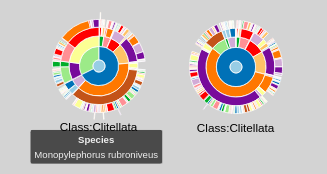
\includegraphics[]{interringCompare.png}
  \caption{Comparación de dos clases usando la visualización InterRing}
  \label{}
\end{figure}

Como se puede observar en la figura 3, es posible detectar diferencias entre las figuras que representan una misma clase (\emph{Clitellata})
mediante las variaciones existentes en ambas figuras, de esta manera se espera poder contribuir con el trabajo de refinamiento de las taxonomías al 
resaltar y hacer más evidentes las diferencias entre versiones de una taxonomía.

Como detalles del modelo propuesto en la extensión del sistema Diaforá podemos listar:

\begin{itemize}
  \item \textbf{Gráficas InterRing:} Se agregan un par de gráficas circulares para representar los árboles taxonómicos de las
  dos versiones de la taxonomía que se está comparando.
  \item  \textbf{Soporte interactivo:} Las gráficas además de representar visualmente los árboles taxonómicos permiten la navegación interactiva
  por parte del usuario. Permitiendo escoger algún nivel específico en el árbol, lo que de manera automática se ve reflejado en la gráfica \emph{edge drawing}.
  \item \textbf{Etiquetas interactivas:} Utilizando el control \emph{Lens} se incluyen etiquetas interactivas que permiten saber cuantas diferencias y de que tipo existen
  en cada uno de los niveles del árbol taxonómico.
\end{itemize}

\subsection{Caso de Uso: \emph{Orden: Haplotaxida}}
Utilizando el sistema \emph{Diaforá} para analizar el órden taxonómico \emph{Haplotaxida} correspondiente al filo \emph{Annelida} \cite{nguyen_nguyen_tran_blakemore_2016}.
En la figura 4 podemos apreciar la comparación entre la versión de la taxonomía del año 2012 y la versión de la taxonomía de 2019 del Catalogue of Life \cite{catalogueoflife}.
\begin{figure*}[]
  \centering
  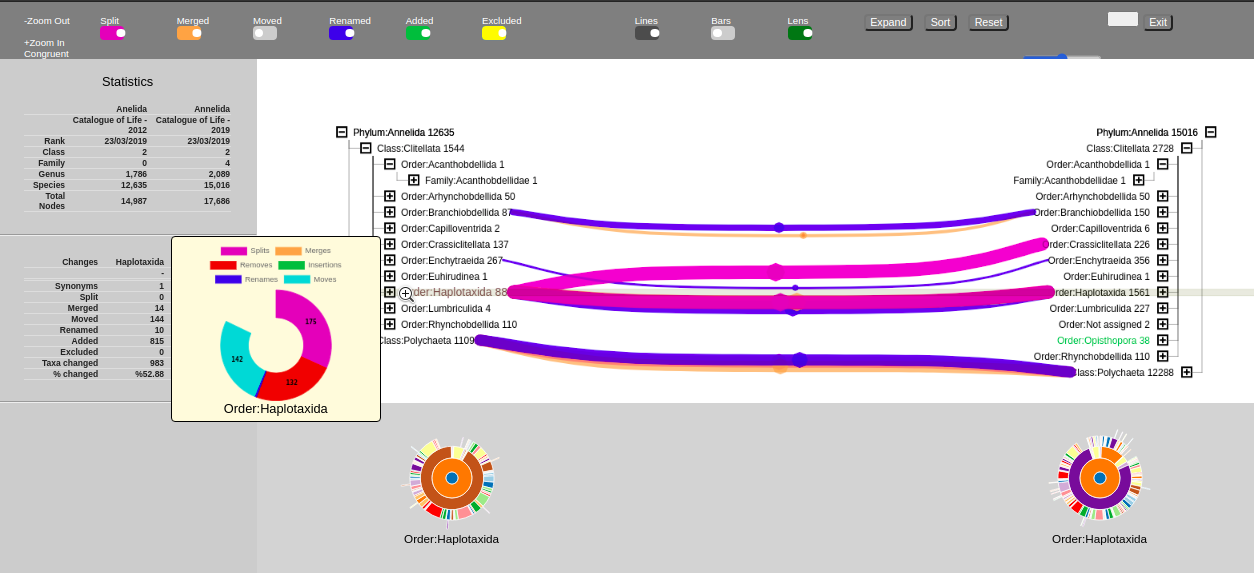
\includegraphics{useCaseHaplotaxida.png}
  \caption{Caso de uso: Orden Haplotaxida}
  \label{}
\end{figure*}

Como es posible apreciar en el resumen de las etiquetas interactivas el órden \emph{Haplotaxida} tiene al menos 175 \emph{splits} o divisiones de los taxones del grupo.
Y eso se refleja adecuadamente en las diferencias de la gráfica \emph{InterRing} en la parte inferior del área de comparación.


Es importante destacar, la sincronía existente entre las gráficas \emph{InterRing} y el árbol taxonómico con \emph{edge drawing}, por lo que cuando el usuario 
selecciona un nodo en alguna de las dos visualizaciones se refleja en la otra para tener en todo momento el contexto del sub-árbol que esta siendo sujeto de comparación.


\subsection{Posibles extensiones a futuro del sistema \emph{Diaforá}}

Se recomienda como posibles temas de extensión al sistema, la posibilidad de incoporar la edición 
de las taxonomías biológicas en el sistema, así como la incorporación de un módulo de análisis de diferencias
que incluya el resumen de los cambios y un conjunto alternativo de visualizaciones incluyendo una visualización matricial
de los datos.

\subsection{Detalles del desarrollo de la herramienta}
El desarrollo al que hace referencia este documento es una extensión del sistema \emph{Diaforá}\cite{sancho_diafora}.
El sistema original esta desarrollado como una aplicación web, 
haciendo uso de la librería Processing \cite{p5js2020}.
Los componentes adicionales que corresponden a la visualización de la gráfica \emph{InterRing} y las etiquetas
interactivas están desarrolladas haciendo uso de la librería Data Driven Documents \cite{DDD}.

Al ser una aplicación web, se permite un fácil acceso y disponibilidad para el uso de los taxónomos y se admite el 
mismo formato de árbol taxonómico que en la versión previa del sistema \emph{Diaforá}.

La aplicación se encuentra publicada en el url: \underline{https://diafora2.herokuapp.com/} donde se puede acceder y probar las extensiones
mencionadas al sistema \cite{Diaforá}.

Los archivos que contienen las taxonomías siguen el formato original de la primera versión del sistema \cite{sancho_diafora}.


\section{Validación del modelo propuesto}
En esta sección se muestran una serie de evaluaciones que realizaron distintas personas para validar que el modelo de 
visualización propuesto cumple con los requisitos para que los taxónomos 
tengan una visualización más adecuada de las taxonomías a la ya existente.
\newline
\begin{itemize}
  \item \textit{“La clasificación en relaciones filogenéticas es la principal función de un taxónomo, para realizar el trabajo de una manera más rápida y eficiente, es necesario herramientas visuales para un mejor rendimiento de los datos y obtener formas de simplificar los datos de una forma visual. Cuando se llegan a tener una gran cantidad de datos para un análisis filogenético, es posible que se dificulten determinar las relaciones sin una visualización gráfica, por lo tanto, la utilización de estas visualizaciones, en específico, la herramienta “InterRing”, tiene mucha utilidad en estos casos. \\ 
  Esta herramienta permite al taxónomo tener una claridad mayor en los datos seleccionados, ya que no requiere que haga “scroll”, y pueda explorar en otras ramas del árbol taxonómico”.}
  
Biólogo BSc. André Leandro C. \\

  \item Evaluación 2.\\
\end{itemize}

\section{Trabajo Futuro}

Para un departamento de IT el concepto de aprovisionar de forma manual o automatizada una infraestructura para un sistema de cómputo \cite{aut-cloud-prov}, termina siendo el conjunto de tareas que tratan en preparar un conjunto de servidores, así como software adicional, configuración de redes, seguridad a la misma y demás, con el fin de ejecutar dentro de ellos aplicaciones de software que realizan distintas tareas, cumpliendo con los múltiples requerimientos dentro de una lógica de negocio.

Tendencias e implementaciones en el campo del aprovisionamiento de infraestructura para sistemas de software ha tomado un giro importante, donde cada vez se le brinda al usuario un mayor aprovisionamiento y menor responsabilidad de la configuración del hardware, el uso de máquinas virtuales \cite{virt-machines} es cosa diaria respecto al lugar donde se ejecutan las aplicaciones, dando paso a procesos de automatización de infraestructura, que quitan aún más la responsabilidad al usuario de preocuparse por temas de hardware.

Modelos recientes sobre infraestructura como código (IaC) \cite{artac-iac} son muy utilizados en aplicaciones en la nube \cite{morris-iac}, donde por medio mayormente de archivos con extensión .yaml, se describen un conjunto de árboles de configuración, las cuales después por medio de herramientas de automatización, se ejecutan todas las tareas deseadas. Desarrollar infraestructura como código \cite{guerr-iac}, \cite{huttermann-iac}, permite la idempotencia en una arquitectura e infraestructura, lo cuál es una enorme ventaja respecto a configuraciones manuales.

Herramientas para Iac como Terraform o Ansible \cite{terraf-ansib} realizan tareas automatizadas para aprovisionar infraestructura y desplegar aplicaciones en dicha infraestructura. Como resultado del aprovisionamiento, Terraform en el fondo utiliza la Teoría de Grafos \cite{Aldous-graphs}, \cite{Kamada-graphs} para definir y mantener dicha especificación en código de la infraestructura en tiempo real. 

Existe una configuración en archivos .yaml que define un estado $deseado$ de la infraestructura, Terraform monitorea en tiempo real cual es el estado $actual$ de y realiza por medio de reducción transitiva una diferencia de grafos, con el fin de comparar y saber si existe una mínima diferencia entre dichos estados ($deseado, actual$) y en caso de existir, realizar a cabo una serie de procesos automatizados que ponen de nuevo el estado actual a como se desea que esté la infraestructura en todo momento.

Un ejemplo de esta diferencia de grafos en Terraform junto con el proceso de recuperación, podría ser tener una definición inicial deseada con 5 servidores corriendo en todo momento, si en algún momento un servidor se cae, Terraform va a realizar la comparación entre el estado $deseado$ de la infraestructura (5 servidores) y el estado $actual$ (4 servidores al estar 1 servidor caído) y va a levantar una instancia para volver a tener el estado actual igual al estado deseado.

Una propuesta para continuar con esta investigación sobre visualizaciones para taxonomías biológicas y una posible implementación de dicho modelo, más allá de un prototipo, va muy de la mano con todas estas tendencias de IaC, aplicando un enfoque similar al de la teoría de grafos para comparación de árboles taxonómicos.

Se propone diseñar otra vista para el taxónomo, donde no va a visualizar todo el despliegue de cada árbol en un año distinto, sino que se podría almacenar en un árbol el contenido del $phylum$ del año inicial de la comparación y en otro árbol distinto el contenido del $phylum$ para el siguiente año que se esté comparando. Posterior a eso se puede llevar a cabo una diferencia de árboles y guardar dicha diferencia en un tercer árbol, el cual va a servir para visualizar únicamente los cambios que han surgido en el $phylum$ en los años que esté comparando. 

Dicho árbol posiblemente contenga considerablemente menos información que cualquiera de los árboles previos, al menos que se estén comparando las mismas especies con una diferencia muy marcada de años. De esta manera, se puede contar con la pantalla de visualización actual junto con los InterRing y a la vez con una segunda pantalla donde se muestre la diferencia o los cambios que han habido entre los años, sin mostrar lo que no haya cambiado.

Dicha pantalla podría constar de datos que representen los cambios que hubieron, puede representarse como un único árbol y a la vez se pueden agregar gráficos de InterRing para visualizar la información de una manera distinta. 

\section{Conclusiones}
Después de analizar distintos modelos para visualizar grandes cantidad de información, es recomendable tener más de una forma de visualizar las taxonomías, contar únicamente con dos árboles donde cada uno representa un $phylum$ de la misma especie en distinto año y cada uno de estos árboles se despliega hasta el fondo del mismo, no es la manera más sencilla de comparar una especie de un año a otro, sin embargo es útil para que el taxónomo no pierda el contexto de lo que está viendo. 

Un enfoque que a manera de validación del modelo propuesto nos ha dado valor, es el hecho de utilizar más de un tipo de visualización, donde se tiene la visualización actual con el desglose total del $phylum$ en distintos períodos, una visualización de InterRing que permite tener de entrada una comparación más abstracta donde más rápidamente podemos ver si han habido cambios, a esto uniéndole la diferencia de grafos de árboles, el taxónomo no depende de una única pantalla para realizar comparaciones, sino que puede optar con distintas pestañas que pueden reducir las comparaciones.

Además, de distintos modelos estudiados durante la investigación de modelos de visualización, cuando se trata de grandes cantidades de datos los que queremos ver en una pantalla, el modelo InterRing es de los más utilizados, dando de entrada una visualización donde se le permite al taxónomo ver si existen diferencias sin entrar en detalle.

%\section{Conclusion}
%The conclusion goes here.





% if have a single appendix:
%\appendix[Proof of the Zonklar Equations]
% or
%\appendix  % for no appendix heading
% do not use \section anymore after \appendix, only \section*
% is possibly needed

% use appendices with more than one appendix
% then use \section to start each appendix
% you must declare a \section before using any
% \subsection or using \label (\appendices by itself
% starts a section numbered zero.)
%


%\appendices
%\section{Proof of the First Zonklar Equation}
%Appendix one text goes here.

% you can choose not to have a title for an appendix
% if you want by leaving the argument blank
%\section{}
%Appendix two text goes here.


% use section* for acknowledgment
%\section*{Acknowledgment}


%The authors would like to thank...


% Can use something like this to put references on a page
% by themselves when using endfloat and the captionsoff option.
\ifCLASSOPTIONcaptionsoff
  \newpage
\fi



% trigger a \newpage just before the given reference
% number - used to balance the columns on the last page
% adjust value as needed - may need to be readjusted if
% the document is modified later
%\IEEEtriggeratref{8}
% The "triggered" command can be changed if desired:
%\IEEEtriggercmd{\enlargethispage{-5in}}

% references section

% can use a bibliography generated by BibTeX as a .bbl file
% BibTeX documentation can be easily obtained at:
% http://mirror.ctan.org/biblio/bibtex/contrib/doc/
% The IEEEtran BibTeX style support page is at:
% http://www.michaelshell.org/tex/ieeetran/bibtex/
\bibliographystyle{IEEEtran}
% argument is your BibTeX string definitions and bibliography database(s)
\bibliography{bibliography}



% that's all folks
\end{document}


